% -----------------------------------------------
% Template for SMC 2020
% adapted from previous SMC paper templates
% -----------------------------------------------

\documentclass{article}
\usepackage{smc2020}
\usepackage{times}
\usepackage{ifpdf}
\usepackage[english]{babel}
\usepackage{cite}
\usepackage{amsmath} 
\usepackage{subcaption}
\usepackage{array}
\newcolumntype{C}[1]{>{\centering\let\newline\\\arraybackslash\hspace{0pt}}p{#1}}

%%%%%%%%%%%%%%%%%%%%%%%% Some useful packages %%%%%%%%%%%%%%%%%%%%%%%%%%%%%%%
%%%%%%%%%%%%%%%%%%%%%%%% See related documentation %%%%%%%%%%%%%%%%%%%%%%%%%%
%\usepackage{amsmath} % popular packages from Am. Math. Soc. Please use the 
%\usepackage{amssymb} % related math environments (split, subequation, cases,
%\usepackage{amsfonts}% multline, etc.)
%\usepackage{bm}      % Bold Math package, defines the command \bf{}
%\usepackage{paralist}% extended list environments
%%subfig.sty is the modern replacement for subfigure.sty. However, subfig.sty 
%%requires and automatically loads caption.sty which overrides class handling 
%%of captions. To prevent this problem, preload caption.sty with caption=false 
%\usepackage[caption=false]{caption}
%\usepackage[font=footnotesize]{subfig}


%user defined variables
\def\papertitle{DIGIDRUM - A HAPTIC-BASED VIRTUAL REALITY MUSICAL INSTRUMENT AND A CASE STUDY}
\def\firstauthor{Silvin Willemsen}
\def\secondauthor{Anca-Simona Horvath}
\def\thirdauthor{Mauro Nascimben}

% adds the automatic
% Saves a lot of output space in PDF... after conversion with the distiller
% Delete if you cannot get PS fonts working on your system.

% pdf-tex settings: detect automatically if run by latex or pdflatex
\newif\ifpdf
\ifx\pdfoutput\relax
\else
   \ifcase\pdfoutput
      \pdffalse
   \else
      \pdftrue
\fi

\ifpdf % compiling with pdflatex
  \usepackage[pdftex,
    pdftitle={Digidrum - A Haptic-Based Virtual Reality Musical Instrument and a Case Study},
    pdfauthor={\firstauthor, \secondauthor, \thirdauthor},
    bookmarksnumbered, % use section numbers with bookmarks
    pdfstartview=XYZ % start with zoom=100% instead of full screen; 
                     % especially useful if working with a big screen :-)
   ]{hyperref}
  %\pdfcompresslevel=9

  \usepackage[pdftex]{graphicx}
  % declare the path(s) where your graphic files are and their extensions so 
  %you won't have to specify these with every instance of \includegraphics
  \graphicspath{{./figures/}}
  \DeclareGraphicsExtensions{.pdf,.jpeg,.png}

  \usepackage[figure,table]{hypcap}

\else % compiling with latex
  \usepackage[dvips,
    bookmarksnumbered, % use section numbers with bookmarks
    pdfstartview=XYZ % start with zoom=100% instead of full screen
  ]{hyperref}  % hyperrefs are active in the pdf file after conversion

  \usepackage[dvips]{epsfig,graphicx}
  % declare the path(s) where your graphic files are and their extensions so 
  %you won't have to specify these with every instance of \includegraphics
  \graphicspath{{./figures/}}
  \DeclareGraphicsExtensions{.eps}

  \usepackage[figure,table]{hypcap}
\fi

%setup the hyperref package - make the links black without a surrounding frame
\hypersetup{
    colorlinks,%
    citecolor=black,%
    filecolor=black,%
    linkcolor=black,%
    urlcolor=black
}


% Title.
% ------
\title{\papertitle}

% Authors
% Please note that submissions are NOT anonymous, therefore 
% authors' names have to be VISIBLE in your manuscript. 
%
% Single address
% To use with only one author or several with the same address
% ---------------
%\oneauthor
%   {\firstauthor} {Affiliation1 \\ %
%     {\tt \href{mailto:author1@smcnetwork.org}{author1@smcnetwork.org}}}

%Two addresses
%--------------
% \twoauthors
%   {\firstauthor} {Affiliation1 \\ %
%     {\tt \href{mailto:author1@smcnetwork.org}{author1@smcnetwork.org}}}
%   {\secondauthor} {Affiliation2 \\ %
%     {\tt \href{mailto:author2@smcnetwork.org}{author2@smcnetwork.org}}}

% Three addresses
% --------------
 \threeauthors
   {\firstauthor} {Multisensory Experience Lab \\ CREATE, Aalborg University\\ Copenhagen, Denmark \\ %
     {\tt \href{mailto:sil@create.aau.dk}{sil@create.aau.dk}}}
   {\secondauthor} {Research Laboratory for Art and Technology \\ KOM, Aalborg University\\ Aalborg, Denmark \\ %
     {\tt \href{mailto:ancah@hum.aau.dk}{ancah@hum.aau.dk}}}
   {\thirdauthor} {Augmented Cognition Lab \\ CREATE, Aalborg University\\ Copenhagen, Denmark \\ %
     {\tt \href{mailto:mana@create.aau.dk}{mana@create.aau.dk}}}


% ***************************************** the document starts here ***************
\begin{document}
%
\capstartfalse
\maketitle
\capstarttrue
%
\begin{abstract}
This paper presents DigiDrum -- a novel virtual reality musical instrument (VRMI) which consists of a physical drum augmented by virtual reality (VR) to produce enhanced auditory and haptic feedback. We present the design and implementation of the instrument-setup together with the preliminary results of a user study which investigates user's haptic perception of the material stiffness of the drum membrane. We test whether tension in the membrane simulation and sound damping (how fast the sound dies out) change the user’s perception of membrane stiffness. We find that higher values for both tension and damping give the illusion of higher material stiffness in the drum membrane, where the sound damping appears to be the more important factor. Our ultimate goal is twofold: on the one hand we seek to create an instrument which allows for enhanced musical expression possibilities through VR. On the other hand, we seek to investigate how haptics influence user interaction in VRMIs and present a preliminary study on this.
\end{abstract}


\section{Introduction}\label{sec:introduction}
Virtual Reality (VR) is described as an immersive environment provided by technology and experienced through sensory stimuli \cite{Serafin:2017}. In VR, one's actions partially determine what happens in the environment. 

Different types of technologies are available for creating VR experiences, and head-mounted displays (HMDs) are among the most popular. VR has been used as a platform for the creation of perceptual illusions, and much research has gone into producing realistic or otherwise compelling visual and auditory experiences. By comparison, the sense of touch has been neglected in spite of its obvious potential to increase a sense of presence in a simulated world \cite{Serafin:2017}.

Virtual musical instruments (VMIs) are defined as software simulations or extensions of existing musical instruments with a focus on sonic emulation. Virtual reality musical instruments (VRMIs), are those which also include a simulated visual component \cite{Serafin:2016}. 

In this paper we describe the design and evaluation of DigiDrum -- a novel VRMI where a single physical drum is enhanced by VR. The user wears a HMD putting her / him in a recording studio where a virtual drum is aligned with the physical drum, i.e., both drums are played at the same time. Interaction with the drum triggers a physical simulation of a drum membrane. The output sound is sent through headphones for auditory feedback. The same sound actuates a vibration motor (haptuator) attached to the inside of a physical drum creating a vibrotactile response in the physical drum -- similar to a real membrane.

As the drum's sound is being simulated, its properties can be changed on the fly, something which is impossible to do in the physical world. In an initial user study we conduct on DigiDrum we try to understand which parameters influence the perception of material stiffness by using different combinations of values for: (1) tension in the membrane and (2) damping, i.e, how quickly the sound dies out. We hypothesise that a higher value for both of these parameters will influence the perception of stiffness positively. Namely, higher tension and higher damping (sound dying out faster) will result in users perceiving the drum membrane as being more stiff. We suspect that tension will be the most important parameter in the perception of stiffness. In our test, the auditory and haptic cues are linked, or matching. 

Experiments investigating the connection between haptic and auditory cues and perception on material stiffness include
Avanzini and Crosato's work \cite{avanzini2006} and Passalenti \emph{et al.}  \cite{passalenti2019}. Both these studies use the haptic device PHANTOM\textregistered{} Omni\textsuperscript{TM} (now Touch) \cite{phantom}. Avanzini and Crosato test the influence of haptic and auditory cues on perception of material stiffness separately, but their work does not deal with musical instruments. Passalenti \emph{et al.}'s experiment focuses on guitar strings. Our experiment takes inspiration from these works, and looks specifically at a VR-enhanced drum.

Our research question is:
\vspace{0.2cm}

\centerline{\it Can we change a user's perception of}

\centerline{\it material stiffness in an enhanced drum membrane}

\centerline{\it using auditory and haptic cues?}
\vspace{0.2cm}
\noindent We are curious to understand if there is a correlation between material stiffness perception and the way a user interacts with the drum. 


Our ultimate interests lie in (1) enhancing musical expression possibilities through a novel VRMI, and (2) investigating user's interaction with a VRMI focused not only on the visual and auditory experience, but also on haptics.


The paper is structured as follows: 
Section \ref{sec:haptics} is an introduction to haptic perception. Section \ref{sec:Design_criteria} describes the design criteria used in for DigiDrum. Section \ref{sec:desex} details a few design avenues we explored during the course of this project. In Section \ref{sec:sys} we describe the system overview and Section \ref{sec:unity} details the implementation of the visual virtual environment. In Section \ref{sec:PM}, the physical model sound algorithm is described. 
In Section \ref{sec:exp} a user study looking at the interaction with the setup is presented and preliminary results shown and discussed in Section \ref{sec:resDisc}. Conclusive remarks and future development are made in Section \ref{sec:conc}.


\section{Haptics}\label{sec:haptics}
% \subsection{Introduction}
The sense of touch is the first to develop in humans -- a sense we cannot shut down. Vision is the last sense to develop, a sense we are able to ``turn off" \cite{Barnett1972} by closing our eyes. Despite this, tactile awareness generally receives less attention than other sensory modalities when it comes to technological development \cite{Gallace2012}. We live in a world over-saturated by visuals, and VR is a technology where this has been the case notably. One reason for the under-evaluation of tactile stimuli could be the broad number of sensations touch comprises: pressure, temperature, pleasure, pain, joint position, muscle sense, and movement. %The experiment we are going to introduce requires subjective evaluation of drum skin vibration in form of a circular membrane. 
In this section, we describe in further detail haptic perception and how it works from a neurophysiological point of view as well as the basis for subjective decision making on tactile sensation.

\subsection{Haptic Perception}
The peripheral nervous system gathers environmental stimuli in form of visual, audible, tactile, olfactory (smell) and gustatory (taste) inputs and transfers them to the central nervous system for further elaboration and integration. Tactile information is collected by proprioceptors in the skin, muscles, and joints and sent to the primary somato-sensory cortex (post-central gyrus) via the dorsal column-medial lemniscus pathway to the thalamic nuclei \cite{Blatow2007}. This cortical area is the first stage for the tactile awareness occurring across body surface. The primary somato-sensory cortex represents tactile stimuli following an inverted order from the toe to mouth \cite{Narici1999}. Several other structures of the central nervous system take part in the generation of tactile feedback, as generally, a single brain area is never responsible for information awareness \cite{Manzoni1986}. Directly connected with the primary somato-sensory cortex is the secondary somato-sensory cortex, an associative area important in humans for light touch and tactile attention \cite{Eickhoff2005}. Literature reports that people undergoing tactile training improve their perception but also strengthen the connections and cortical representations of the stimulated body area \cite{Saito2007} with a direct relationship between size of cortical region and haptic performance. A specific area of the central parietal lobe, placed in the back of the primary somatosensory cortex, integrates the information from the visual and haptic regions to locate objects in space. 

\subsection{Notes on Experiments Involving Haptics}
Conducting experiments on haptics can prove difficult because there are no proper technological devices for delivering controlled and reliable tactile stimuli \cite{Gallace2012}. In virtual environments (as used in VR) and using hand tracking devices such as Leap Motion \cite{leapwebsite} (see Section \ref{sec:sys}), subjects are able to move their hands freely, which could confound somato-sensory processing with activations related to motor planning and movement \cite{Bodegard2001}. These uncontrolled motor activities result in uncontrolled somatic stimulation. There is an anatomical explanation of this close somato-motor functional relationship: areas involved in the perception of touch on the hands in the primary somato-sensory cortex are located mostly in front of the areas responsible for hand movements \cite{Penfield1950}.
Another problem with haptics is the subjective quantification of the stimuli. Contents of tactile consciousness vary between individuals and a common lexicon to evaluate haptic sensation through surveys still seems far to be conceived \cite{Gallace2010}.

\subsection{Interaction between Visual Information and Tactile Feedback}
In a famous experiment, Pavani \emph{et al.} \cite{Pavani2000},  asked a group of participants to detect the position of vibro-tactile stimuli on their arm. The participant's own arm was placed under a table (out of sight) while a fake rubber hand was laid in front of them. The rubber hand was laid out in a position that was anatomically compatible with participant's real hand. When seeing the mannequin hand being touched, all participants reported that their own hand was being touched, even though that was not the case. In short, the perception of tactile stimulation was simulated through visuals. A similar experiment was conducted by \cite{Schaefer2006} asking subjects to watch a video of a hand being touched on the first finger while their own hand was stimulated synchronously. Brain activity during synchronous stimulation showed an improved tactile acuity. Taking into account previous literature findings, we can conclude that in virtual environments hand manipulations and interactions are important factors that enhance realism and user experience. 


\section{Design Criteria}\label{sec:Design_criteria}

In designing DigiDrum we look at design criteria for VRMIs suggested by Serafin \emph{et al.} \cite{Serafin:2016} and try to accommodate as many recommendations as we can in our implementation. We create a setup which integrates visuals, sound and haptics and extend an existing musical instrument using VR seeking to create a ``magical interaction". We try to create a sense of presence by mapping a virtual drum's location to that of a physical one, and by representing the user's hands in the simulated world. We seek to create three types of illusions with our installation: a place illusion -- users should feel like they are in a music production studio, a plausibility illusion -- users should feel like the experience is really happening, and virtual body ownership -- users should see their own body in the virtual world and feel ownership of their virtual body.

\section{Design Explorations}\label{sec:desex}
Re-creating the user's hands in the virtual world is an important aspect in the design of an enhanced drum. During the design development process of this project, we explored two different ways of tracking users' hand movement in the virtual world: (1) the Myo armband -- a device which tracks forearm movement, converting muscle activation to electric potentials and (2) the Leap Motion -- a device which can track and reconstruct a user's hands in VR. We chose the latter for our implementation and this section will briefly explain our decision. 

The Myo (by Thalmic Labs, now North) \cite{northwebsite} is a wireless sensor that records surface electromyographic (sEMG) activity from 8 sensors placed around the forearm. Sensors record EMG signals converting muscle activation in electric potentials. The Myo can detect the forearm movement in space, flexion and extension of the wrist and when a subject is spreading the fingers or closing the fist. %The sampling frequency of the device is 200 Hz and the signal amplitude is expressed in “units of activation” and not in millivolts (mV) like standard electromyographic recorders. The armband encloses a nine axis inertial measurement unit which contains a three axis gyroscope, three axis accelerometer and a three axis magnetometer \cite{northwebsite}. From these measurements of spatial information, the wearer’s arm can be tracked both in the orientation and movement. The orientation data indicates the positioning of the armband in terms of the euler angles (roll, pitch and yaw). The angular velocity of the armband is provided in a vector format and the accelerometer represents the acceleration the Myo armband is undergoing at a given time. It should be considered that the Myo armband is better suited for determining the relative positioning of the arm rather than the absolute position. The Myo armband has been made to work best at the widest part of the forearm, that is, the upper forearm %(\autoref{fig:arm1})
% \begin{figure}[h]
% 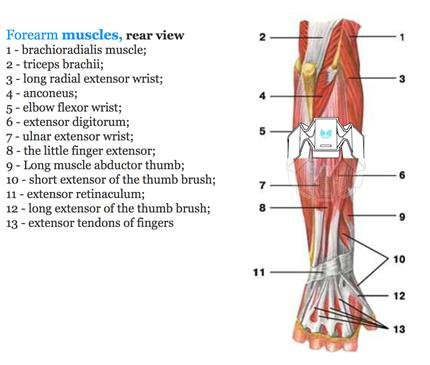
\includegraphics[width=0.5\textwidth]{myo_armband_muscles}
% \caption{Muscle detected and armband position}
% \centering
% \label{fig:arm1}
% \end{figure}
% The Myo can detect the forearm movement in space, flexion and extension of the wrist and when a subject is spreading the fingers or closing the fist. 
% \subsection{Raw signals and pre-processing for the Myo Armband}
% To obtain gestural data from a subject after wearing the armband it is possible to extract the raw signals as shown in \autoref{fig:signals} (a). The armband uses a bluetooth connection to stream data to the PC for data collection and interpretation. It is suggested “warm-up” the band following the app's procedure before starting to collect sEMG signals.
% % \begin{figure}[h]
% % \includegraphics[width=0.5\textwidth]{signals0}
% % \caption{Raw sEMG signals as extracted from Myo armband}
% % \centering
% % \label{fig:sig0}
% % \end{figure}

% However, as raw signals have limited practical application, after common pre-processing, involving rectification and envelope calculation (see \autoref{fig:signals} (b)), these signals are more easily interpreted and could be integrated in the Unity environment \cite{unity} (see Section \ref{sec:sys}) for hand gesture control. 
% % \begin{figure}[h]
% % \includegraphics[width=0.5\textwidth]{signal1}
% % \caption{Post-processed sEMG signals}
% % \centering
% % \label{fig:sig1}
% % \end{figure}
% In Unity, the armband needs to sit on the subject for at least 2 minutes to be considered “stable”. A simple controller was created using a thin rectangle with a box on the top to simulate a drum-stick. One end-point is fixed in the same way human forearm connects at the elbow. The box changes colour according to wrist movement in extension (green) or flexion (blue). In other positions, the box stays gray. In \autoref{fig:mm1}, the extension of the palm of the hand is detected by the system and the colour of the box turned to green. Using forearm motion and wrist extension or flexion it could be possible to create a virtual drum using collisions with virtual drum parts. When collision between the virtual stick controlled with Myo and the drum component is detected, a sound file could be played with a pre-sampled musical tone. A simple demo was created using this procedure using a cymbal and a snare-drum.

% \subsection{Leap Motion}

The Leap Motion \cite{leapwebsite} is an infrared-sensor-based camera that allows for accurate hand tracking and can be used in VR and AR environments. The sensor can be simply mounted on top of a HMD and, once calibrated, its software development kit (SDK) allows for accurate hand tracking.

Possibly the most important reason for our decision, is that we need to obtain the exact location of the hands, or more specifically, the fingertips, for interaction. The Leap Motion is much better at obtaining this data than the Myo. Theoretically, data from the Leap Motion could be combined with the data from both Myo armband in order to create a full 3D virtual simulation of the forearm, hand and fingers. However, for the first iteration of the DigiDrum, we find that visualisation of ones own hands is sufficient for tactile evaluation of drum interaction.

\begin{figure}[ht]
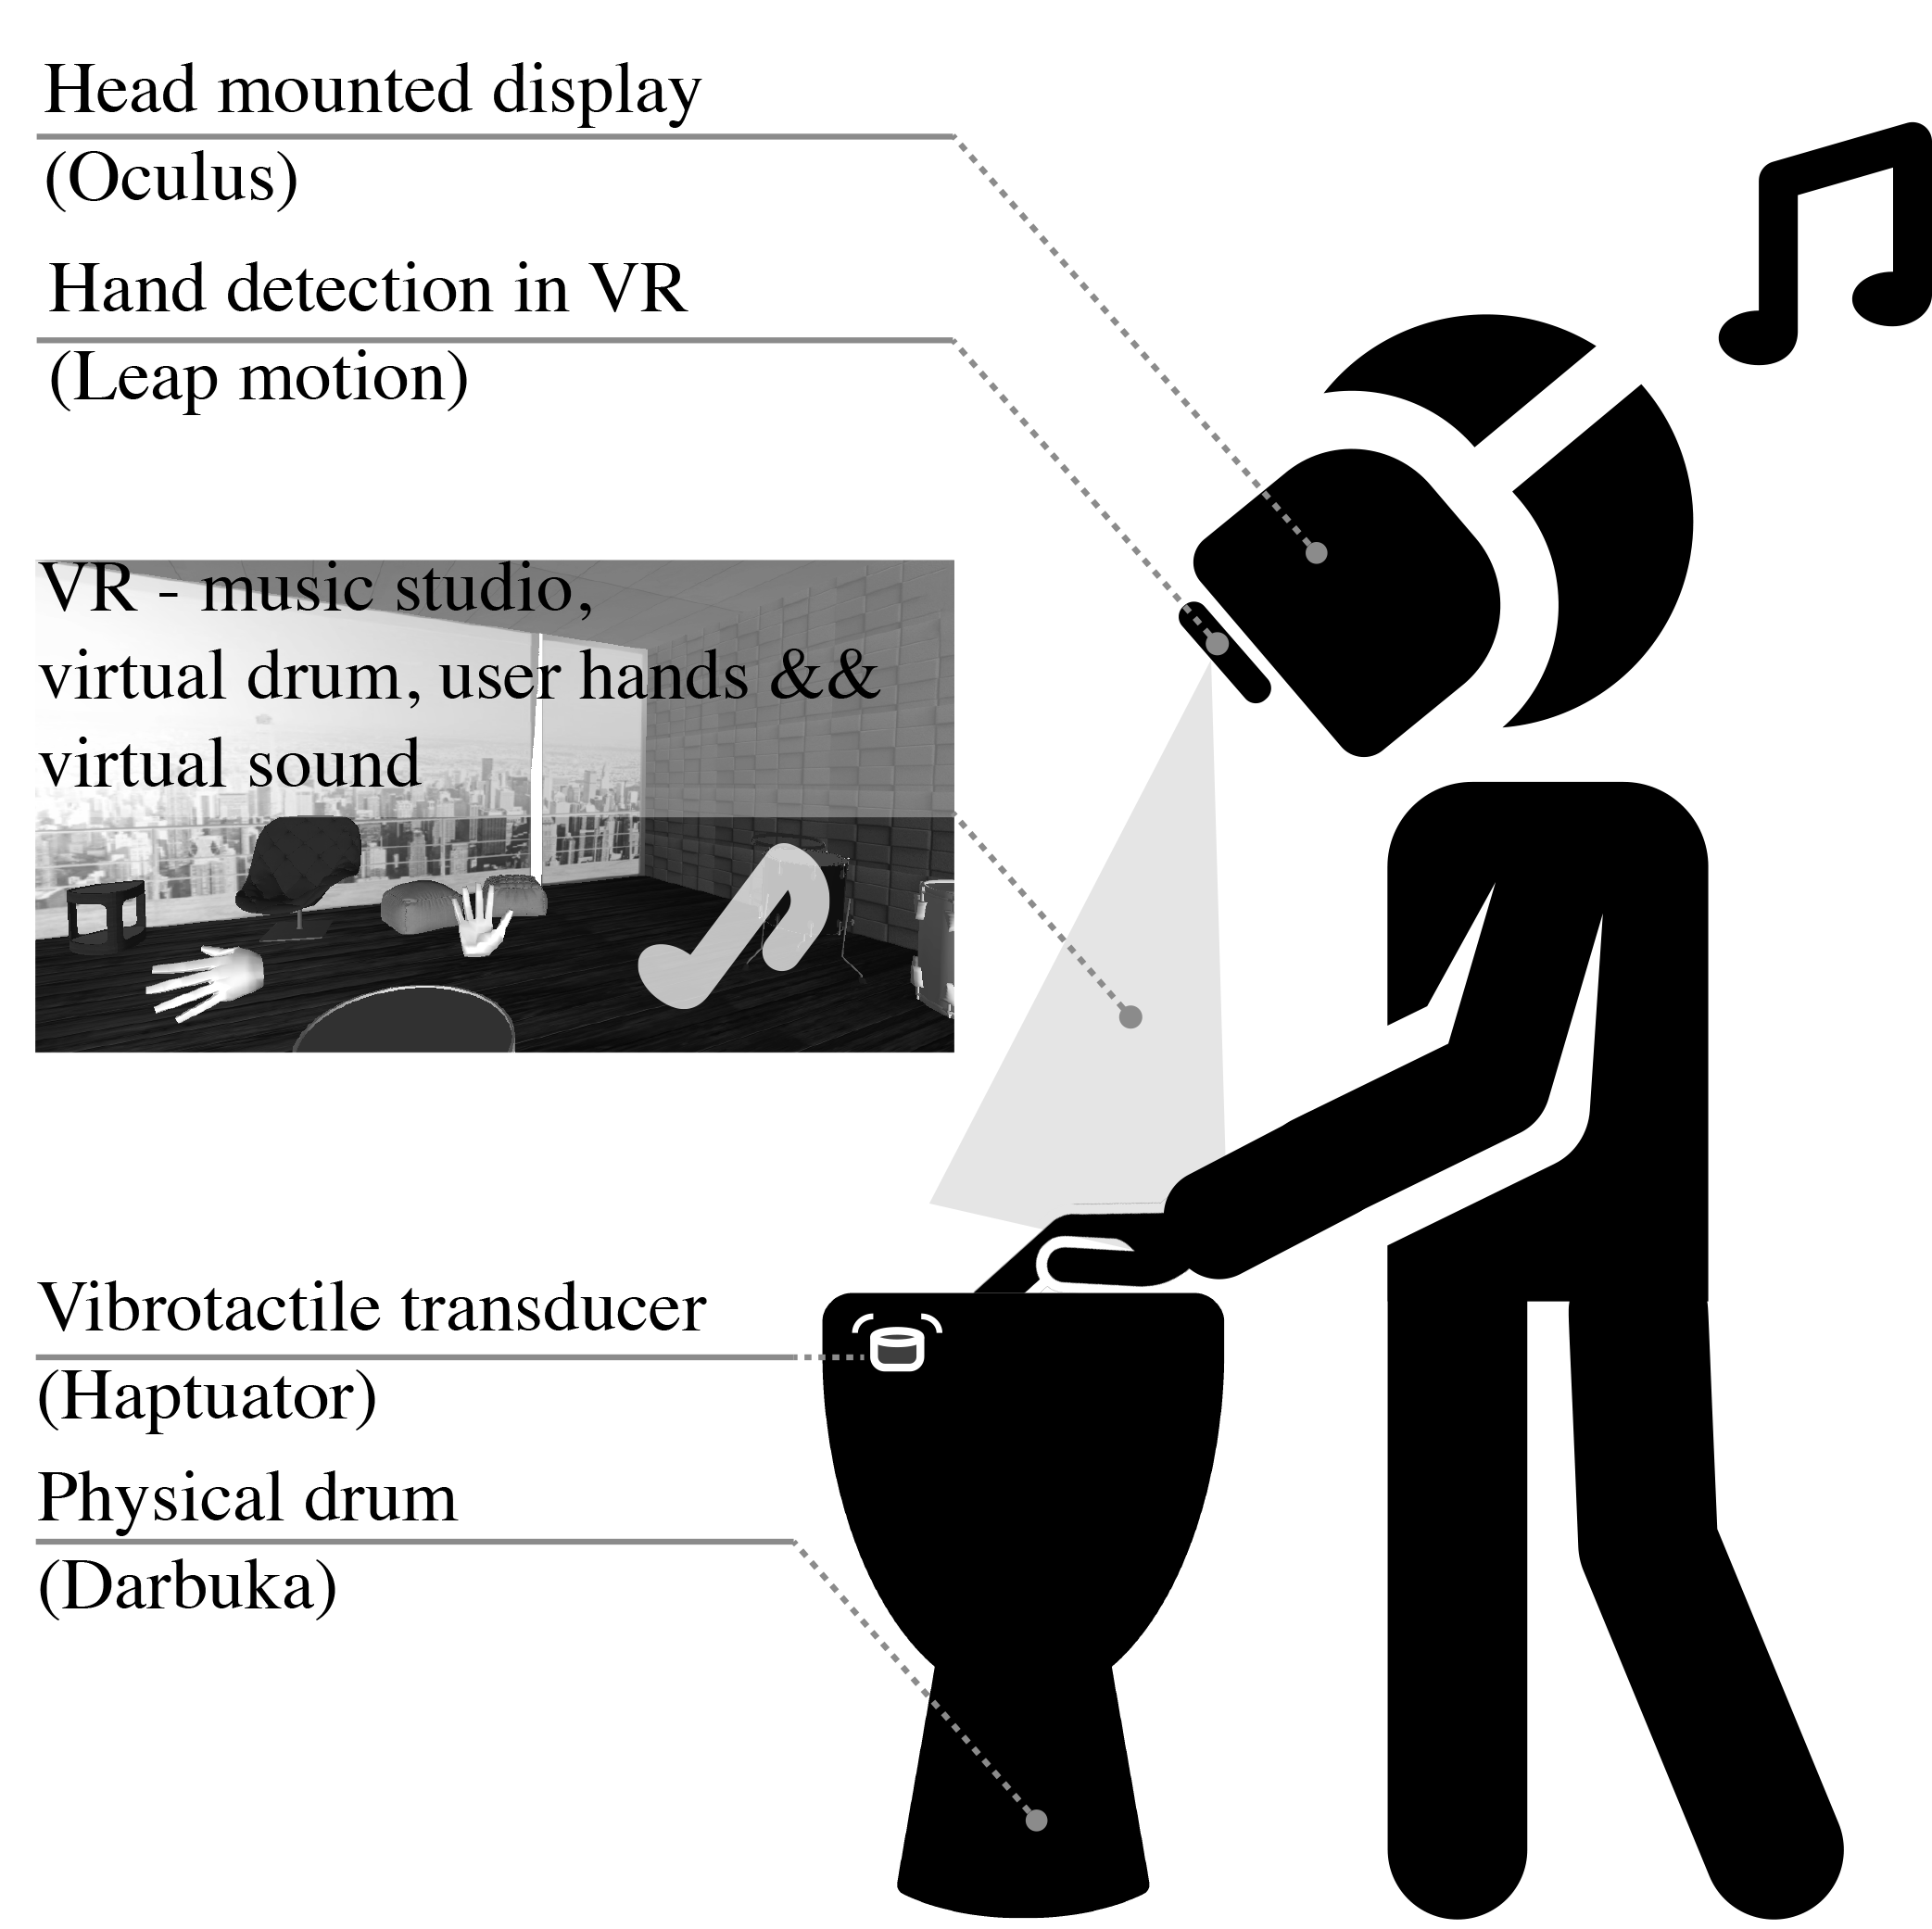
\includegraphics[width=1.0\columnwidth]{SMC 2020 paper template LaTeX/Images/VRDrumSetup.png}
\caption{The physical setup of the system. The Leap Motion is mounted to the front of the HMD.}
\centering
\label{fig:userOverview}
\end{figure}

\begin{figure}[t]
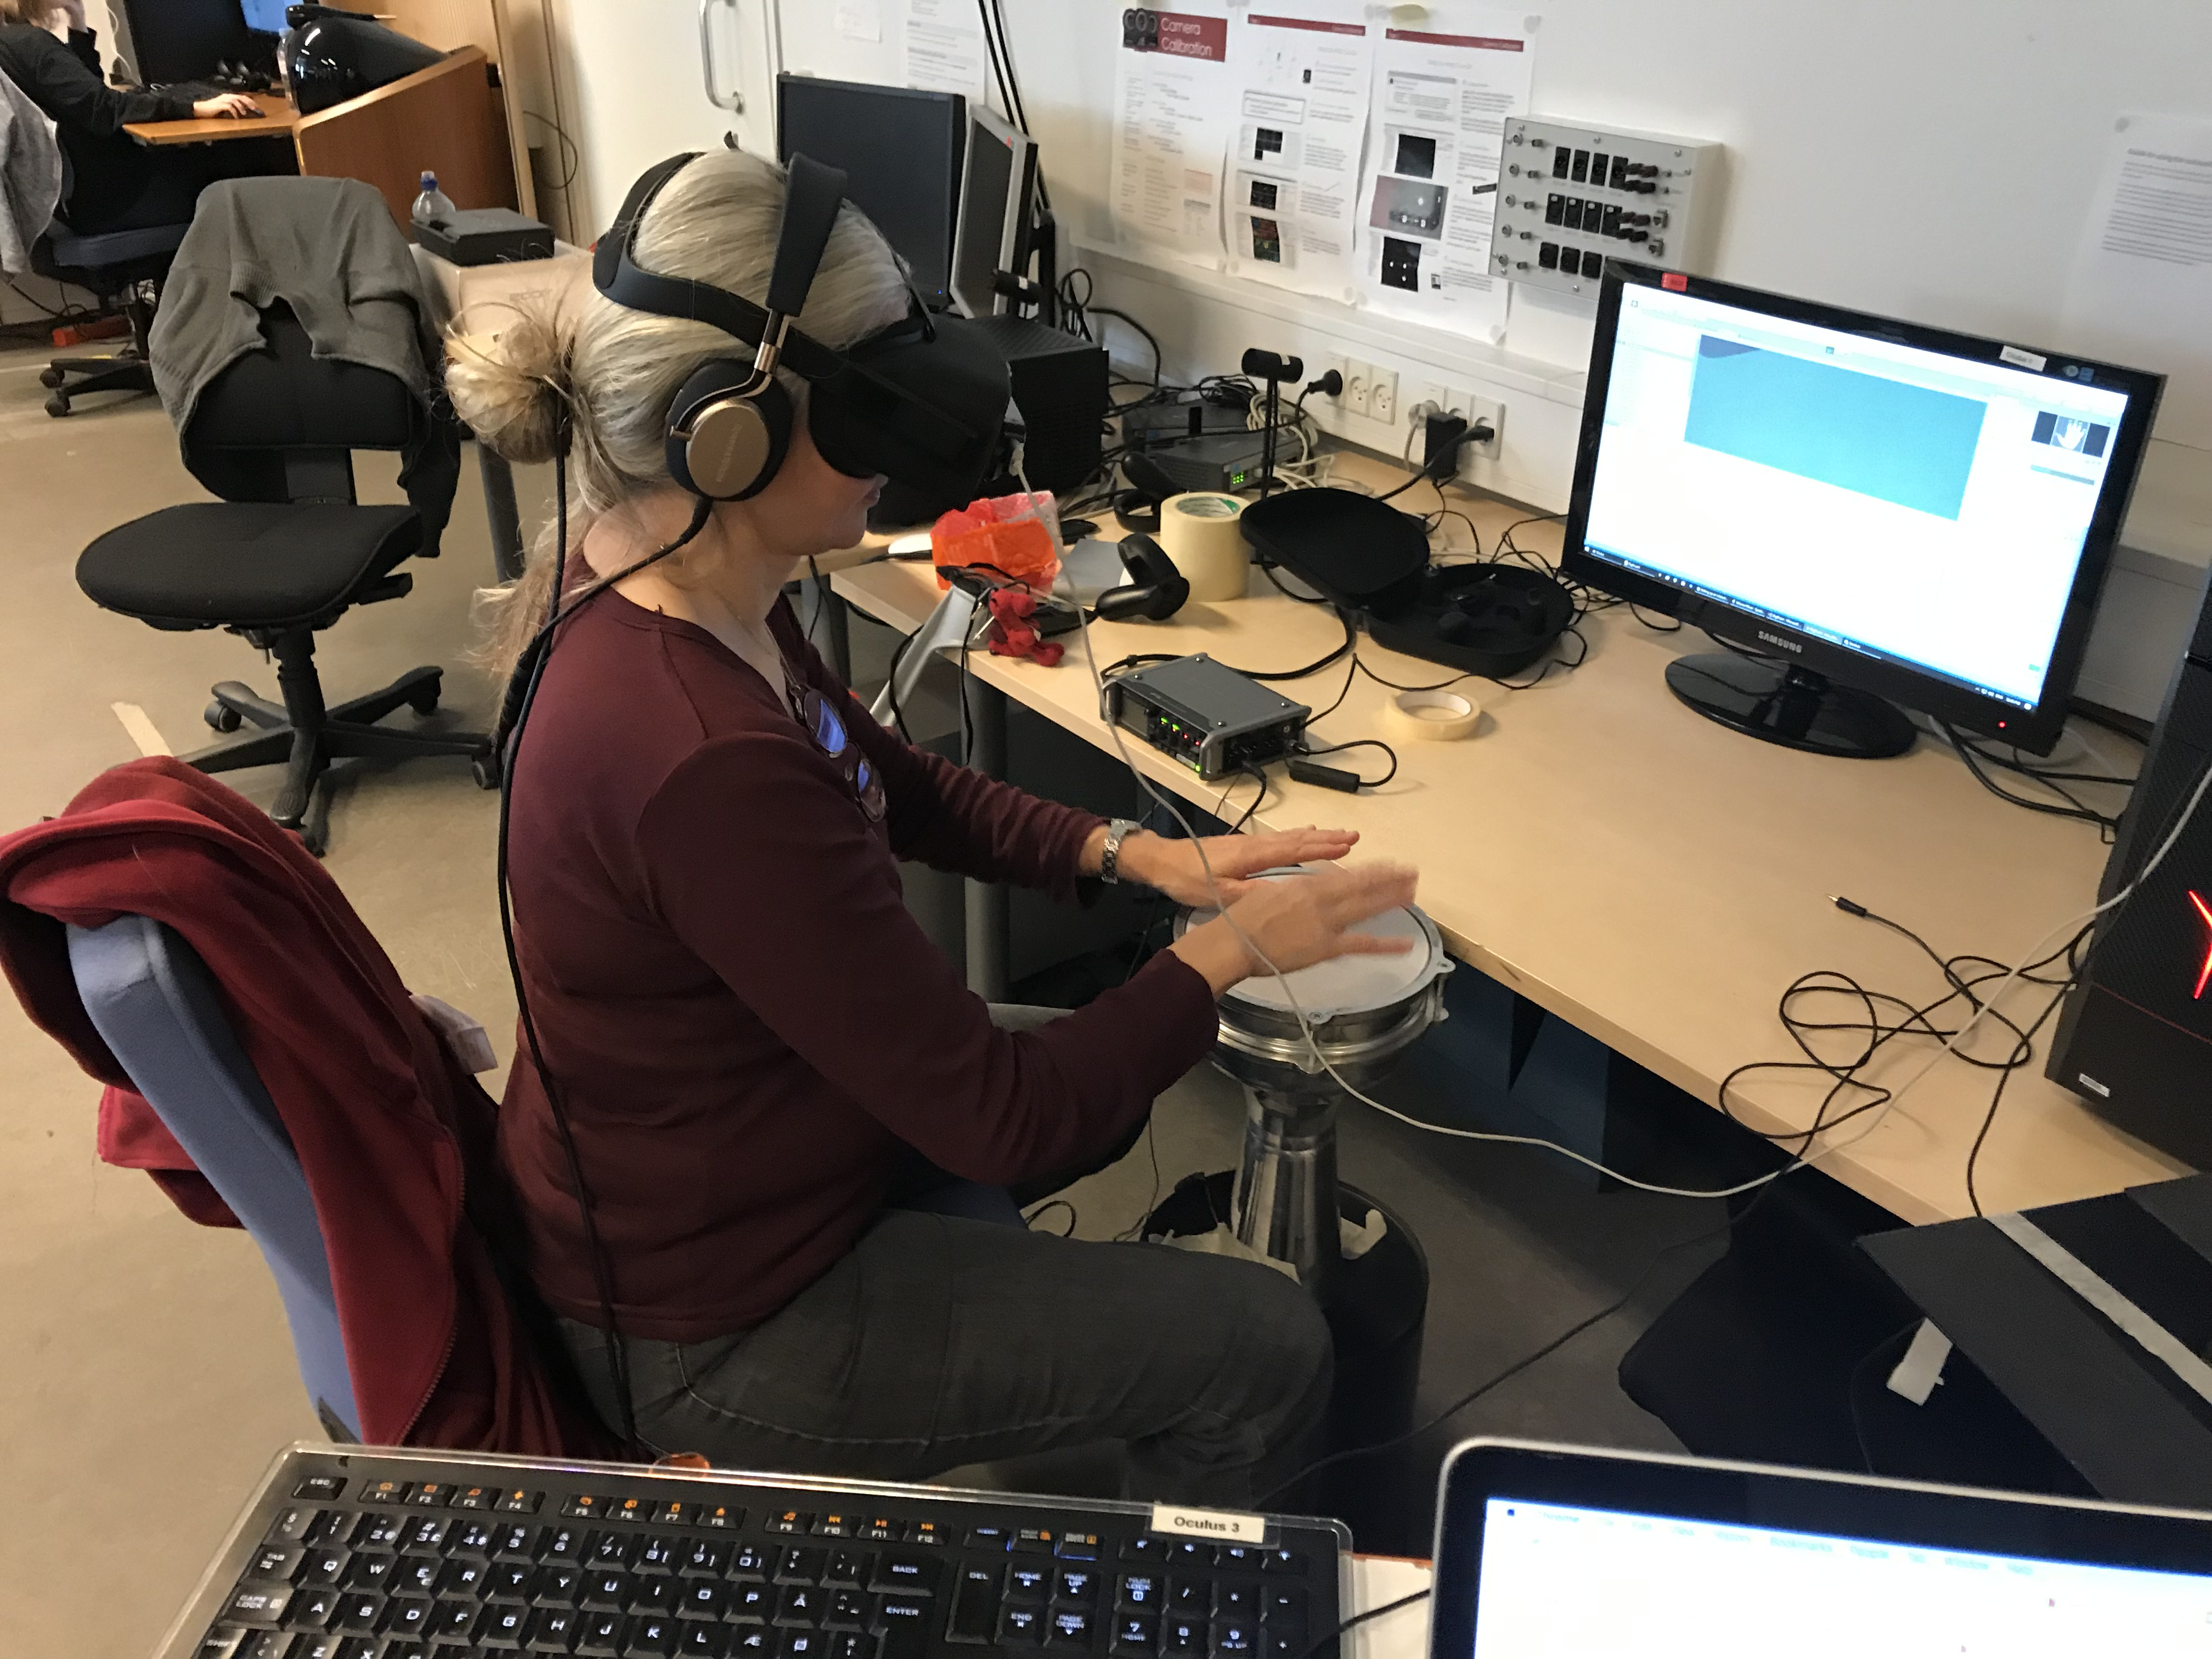
\includegraphics[width=1.0\columnwidth]{SMC 2020 paper template LaTeX/Images/user.jpg}
\caption{A user interacting with the setup.}
\centering
\label{fig:user}
\end{figure}
\begin{figure}[t]
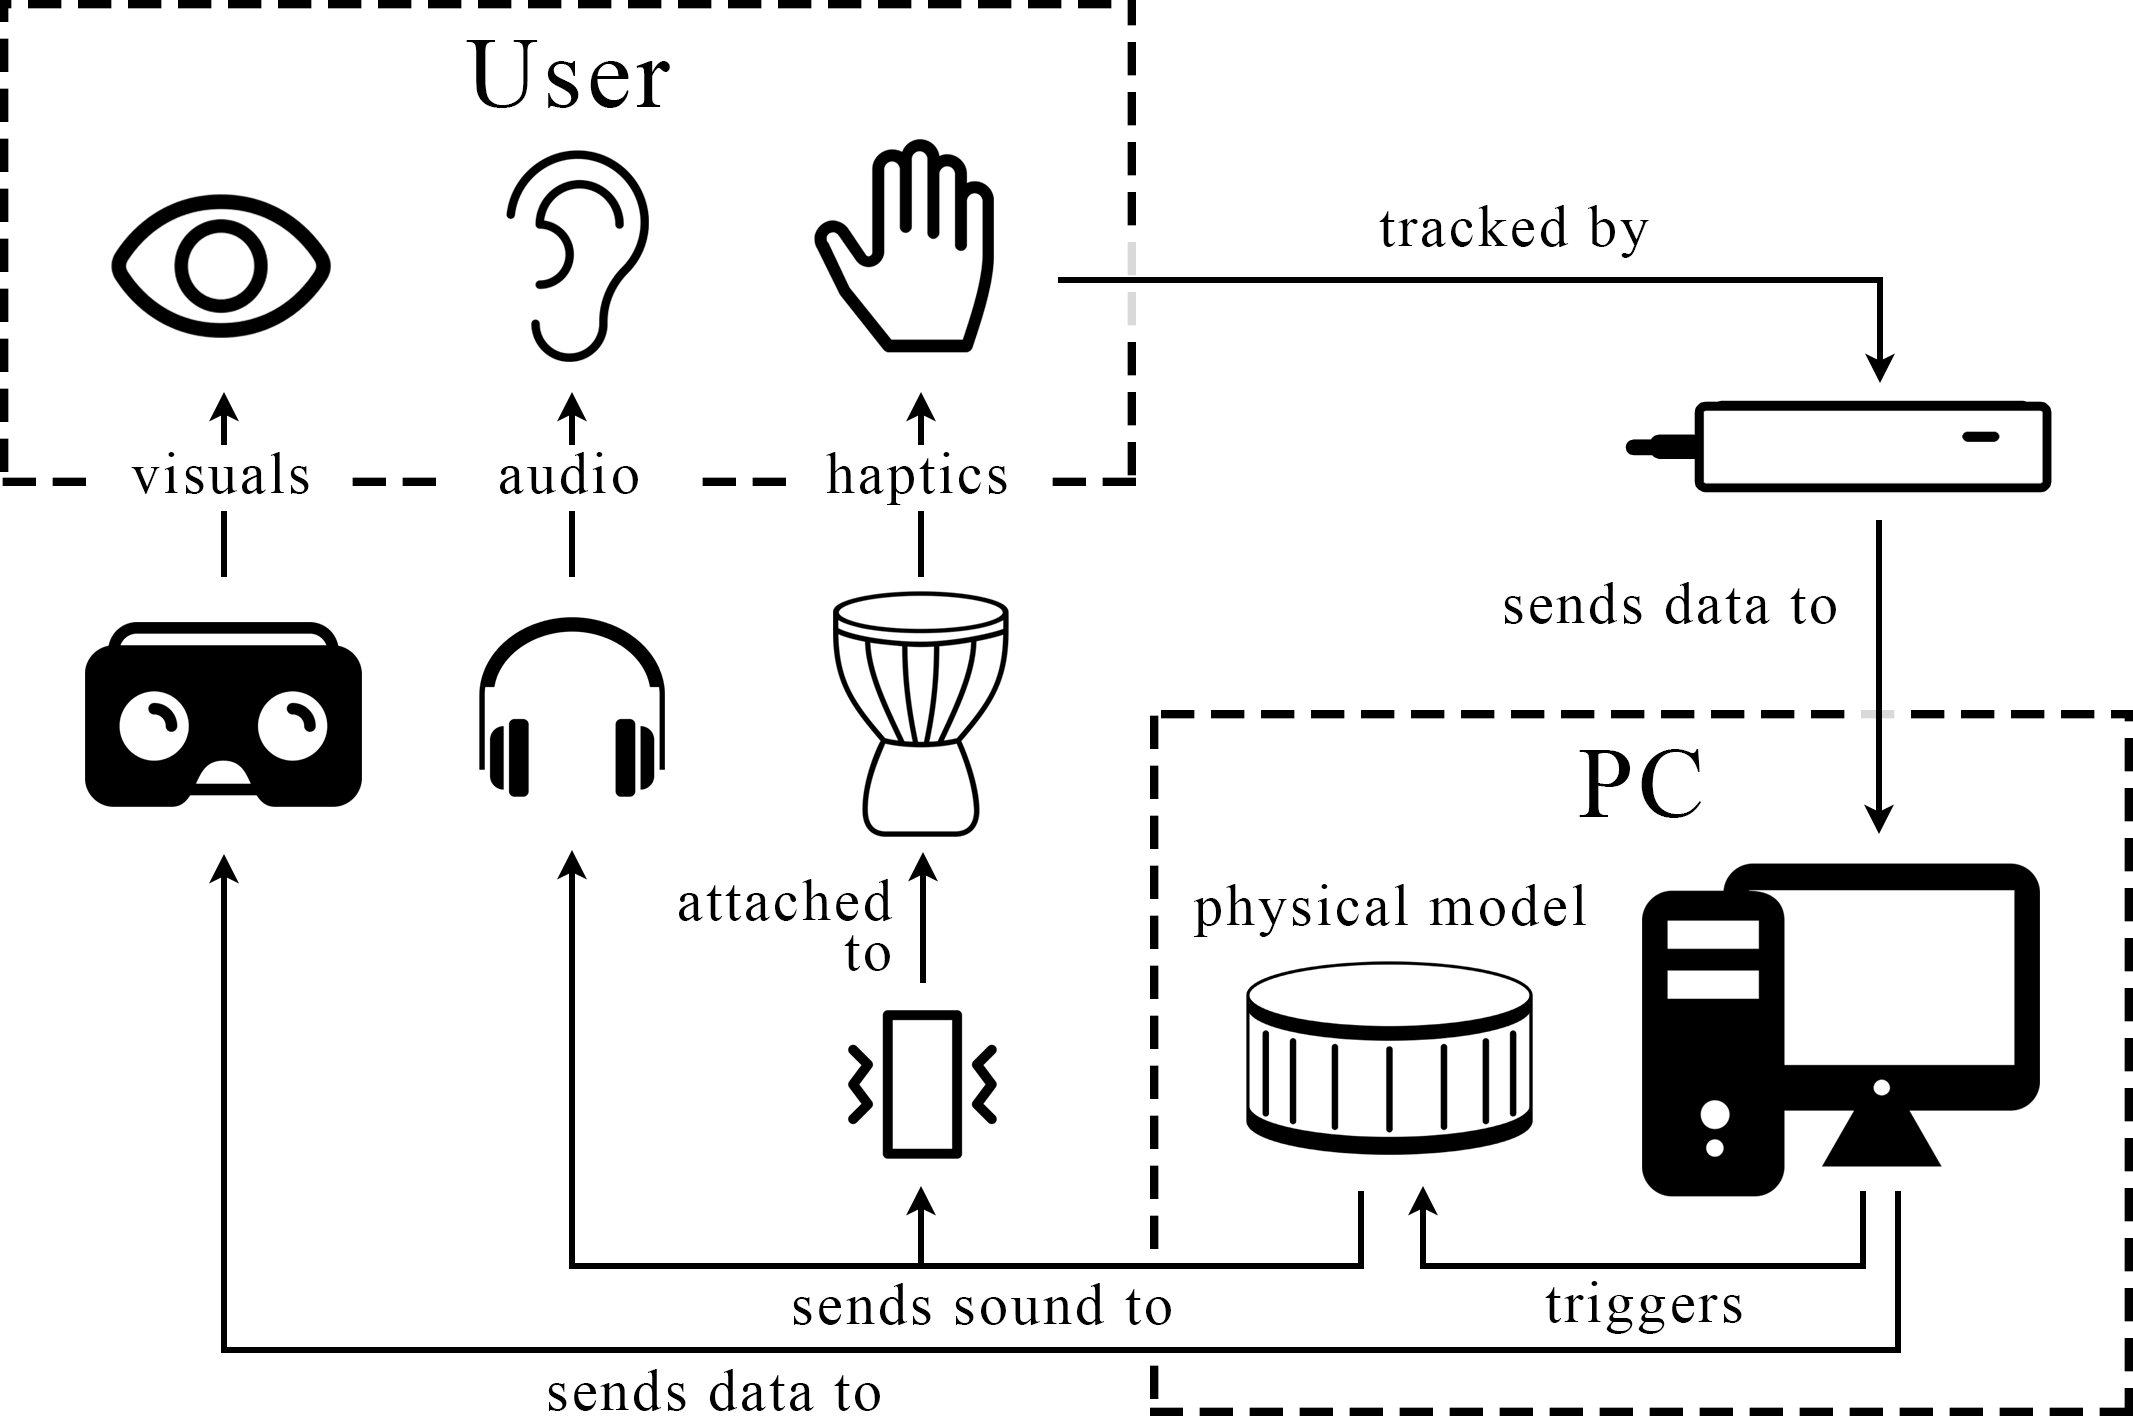
\includegraphics[width=1.0\columnwidth]{Images/systemlayout-updated.png}
\caption{Detailed system layout. The user interacts with the system using their hands and gets haptic feedback from the haptuator attached to the drum membrane, auditory feedback from closed headphones and visual feedback from the Oculus Rift headset. A detailed explanation can be found in Section \ref{sec:sys}.}
\centering
\label{fig:systemLayout}
\end{figure}
\section{System Overview} \label{sec:sys}

\autoref{fig:userOverview} shows the overall design of DigiDrum and its setup and \autoref{fig:user} shows a user interacting with the setup. A Leap Motion tracking sensor is mounted to the front of an Oculus Rift HMD so that hands are always in the ``field of view'' when one looks at the virtual drum. The drum is fixed in-place and played like a djembe. In the application, the virtual drum was placed slightly higher than the physical drum to make sure the physical model was triggered when the physical drum was hit.

A detailed overview of the system is given in \autoref{fig:systemLayout}. The hand movement data is retrieved by a PC which runs the cross-platform game engine Unity \cite{unity}. The Unity scene contains the virtual environment (see Section \ref{sec:unity}) that the user will see through the HMD and the physical model used for the sound and haptics (see Section \ref{sec:PM}). The HMD also sends data back to the PC regarding location and head rotation. Once the tracked hand touches (or collides with) the virtual drum, the physical model is triggered and its output sound is sent to a haptuator which is attached to the inside of the drum membrane using thin double-sided tape. This causes the physical membrane to be actuated by a virtual membrane. The same sound is sent to sound-isolating headphones so that the sound coming from the physical drum does not interfere with the audio coming from the simulated drum.

\section{Unity Implementation}\label{sec:unity}
As mentioned before, the virtual environment is  created using Unity. All the hardware drivers and software components are linked together using this platform. Here, we created a virtual drum playable with hand motion using Leap Motion. The user enters the VR environment (rendered as a recording studio) and Leap Motion reconstructs (in VR) the subject's own hands. In the virtual recording studio we placed a drum at the center. The virtual drum is programmed to detect collision with the reconstructed hands. When a collision was detected, a C\# script, in which a physical model of a drum membrane is programmed, gets activated to reproduce the beating sound of the drum through an actuator placed inside the drum skin.

\section{Physical Model}\label{sec:PM}
The behaviour of musical instruments can be well described by partial differential equations (PDEs) \cite{Fletcher1998}. In this section, the continuous-time PDE for a drum-membrane will be given and explained. This is followed by an explanation of the discretisation method used. Finally, we give the parameter values used for our implementation . 

\subsection{Continuous Time}
A rectangular (stiff) membrane with dimensions $L_x$ (m) and $L_y$ (m) can be described by the following equation \cite{bilbao2009numerical}:

\begin{equation}\label{eq:PDE}
\rho H\frac{\partial^2u}{\partial t^2} = T\Delta u - D\Delta\Delta u - 2 \sigma_0\frac{\partial u}{\partial t} + 2 \sigma_1 \Delta \frac{\partial u}{\partial t}.
\end{equation}
Here, state variable, $u = u(x,y,t)$ is a function of horizontal coordinate $x \in [0, L_x]$, vertical coordinate $y \in [0, L_y]$ and time $t\geq0$ and is parameterised in terms of material density $\rho$ (kg/m$^3$), membrane thickness $H$ (m), tension $T$ (N) and frequency independent and dependent damping coefficients $\sigma_0$ (s$^{-1}$) and $\sigma_1$ (m$^2$/s). Furthermore, $D = EH^3/12(1-\nu^2)$ with Young's modulus $E$ (Pa) and Poisson's ratio $\nu$. Lastly, $\Delta$ represents the 2D Laplacian \cite{bilbao2009numerical}:
\begin{equation}
    \Delta = \frac{\partial^2}{\partial x^2} + \frac{\partial^2}{\partial y^2}.
\end{equation}
Furthermore, clamped boundary conditions -- i.e., the state $u$ at all plate edges and their gradients are 0 -- have been chosen for simplicity:
\begin{equation}
    u = \nabla u = 0 \quad \text{with} \quad \nabla = \frac{\partial}{\partial x} + \frac{\partial}{\partial y}.
\end{equation}
\subsection{Discretisation}
For implementing the physical model, finite-difference time-domain (FDTD) methods have been used \cite{bilbao2009numerical}. This technique discretises $u(x,y,t)$ shown in Equation \eqref{eq:PDE} to $u_{(l,m)}^n$ using $x=lh$ where $l \in [0, ..., N_x-1]$ and $y=mh$ where $m \in [0, ..., N_y-1]$ where $N_x$ and $N_y$ are the number of horizontal and vertical grid points respectively. Furthermore, time is discretised using $t = nk$ with sample $n$ and time step $k$ (s) and $h$ (m) is the space between two grid points can be calculated using 
\begin{equation}\label{eq:h}
    h \geq h_\text{min} =  2\sqrt{\frac{c^2k^2 + 4\sigma_1k + \sqrt{(c^2k^2 + 4\sigma_1k)^2 + 4\kappa^2 k^2} }{2}},
\end{equation}
where $c = \sqrt{T/\rho H}$ and $\kappa = \sqrt{D/\rho H}$. The closer $h$ is to $h_\text{min}$, the higher the accuracy of the implementation.
\subsection{Parameters}
Most parameters used in the simulation were chosen empirically and can be found in \autoref{tab:parameters}. With these parameters we will have a small (30$\times$30 cm) membrane with a low density and stiffness. For the purpose of getting the model to work in real time, the minimum grid spacing $h_\text{min}$ in Equation \eqref{eq:h} is multiplied by 4 ($h_\text{min}$ in \eqref{eq:h} is calculated based on the highest value of $T$ and $\sigma_1 = 0.005$). The values for $T$ and $\sigma_0$ correspond to the cases we are using in the experiment. The frequency dependent damping  $\sigma_1$ follows an exponentially decaying curve, 
\begin{equation}
    \sigma_1(t) = 0.005e^{-0.01 t},
\end{equation}
where $t=0$ at the time of excitation. This allows for very low damping, i.e., very long sound, while taking away some of the high frequency content present immediately after excitation. This ultimately results in a more natural drum sound, even when $\sigma_0$ is set low.
\begin{table}[h]
\caption{Table showing parameter values.}\label{tab:parameters}
\centering
\begin{tabular}{|c|c|c|}
    \hline
    Parameter & Symbol (unit) & Value \\
    \hline
    Membrane width & $L_x$ (m) & $0.3$\\
    Membrane length & $L_y$ (m) & $0.3$ \\
    Material density & $\rho$ (kg/m$^3$)& $10$ \\
    Thickness & $H$ (m) & $0.001$ \\
    Tension & $T$ (N) & $T = \{15, 40, 80\}$ \\
    Young's modulus & $E$ (Pa)& $2\cdot 10^3$ \\
    Poisson's ratio & $\nu$ (-)& $0.3$ \\
    Freq. indep. damping & $\sigma_0$ (s$^{-1}$) & $\sigma_0 \in \{0.5, 2, 5\}$\\
    Freq. dep. damping & $\sigma_1$ (m$^2$/s) & $\sigma_1 \in [0, 0.005]$\\
    Time step & $k$ (s) & $1/44100$\\
    Grid spacing & $h$ (m) & $4h_\text{min}$\\
    \hline
\end{tabular}
\end{table}

\section{Experiment}\label{sec:exp}
%In the above we presented a drum augmented using virtual reality and a vibration motor. Considering that different physical drums would produce different acoustic results our virtual reality musical instrument is an implementation of 3 different drum types into a single setup. While getting the haptic feedback of a drumming experience, one can switch between different musical instruments, explore their potential and train their stroke. 
% DigiDrum should allow for novel ways of musical expression. We now wish to test it in order to understand how we can improve our design, and to see if we were right in focusing on haptic and auditory cues for a VRMI design. Can DigiDrum be used as a tool for informing knowledge on haptic and audio perception?

Through a user study, we inquire how the tension and frequency independent damping coefficient ($T$ and $\sigma_0$ respectively in Section \ref{sec:PM}) influence the perception of material stiffness.
 
Additionally, we hope -- on a larger scale -- to add to the corpus of design guidelines for VRMIs, more specifically those VRMIs which involve a touch based stroking movement. In \cite{Serafin:2016}, Serafin et al. describe three layers of evaluation for VRMIs, namely: (1) investigating modalities of interaction, (2) evaluating VR specific aspects, with engagement being the most interesting from a VRMI perspective, and (3) looking at quality and goals of interaction. The focus of our experiment is on the former -- modalities of interaction.

As shown in Section \ref{sec:PM}, we have 3 different cases for both tension $T$ and frequency independent damping $\sigma_0$. All combinations are tested, resulting in 9 different cases. Participants' experiences are evaluated through (1) asking them during the test how they rate the stiffness of the material in each of the 9 cases, (2) a questionnaire including questions about their relationship and experience with playing a musical instrument, virtual body ownership and whether they thought their interaction patterns changed between the different cases and (3) observation while the participants were interacting with the setup to retrieve data on engagement and stroke patterns which possibly correlate to the haptics and sound.

\subsection{Experiment Process}
Before the experiment, participants were told that they would be ``drumming in VR" and that we would test their perception of the stiffness of the material they are interacting with. They were told that they were going to hear 9 different cases in between which the ``parameters of the experience" would be changed and that for each of these cases they would have to rate the stiffness of the material they were interacting with on a scale of 1 to 7, 1 being ``extremely soft or loose", 7 being ``extremely stiff or hard". The order in which the cases were presented was randomised to reduce bias. Between cases, the participant would not take off the headset or headphones, and we would note their answers. After the test, the participants would fill out a questionnaire with the following questions (the last two taken from \cite{avanzini2006}):

\begin{itemize}
    \item I felt like the hands in the simulation were my own. (1-7 rating)
    \item In order to express your judgements to the questions during the simulation, you relied mainly on... (multiple answers possible: visuals\textbar audio\textbar haptics)
    \item In your opinion what was varying between each condition? (multiple answers possible: visuals\textbar audio\textbar\ haptics)
\end{itemize}
From participant observation during the experiment and the the final two questions of the questionnaire, ``Did your behaviour change between different cases, and if so what did you do differently?" and ``Anything you would like to add?", we hoped to get information on the user interaction and the quality of our setup.

The experiment was done on 16 participants, 9 of which were experienced musicians ($>$ 5 years of instrument practice). Three participants were drummers. 

\section{Results and Discussion}\label{sec:resDisc}
This section will give the results of the user study and discuss these. Due to the small sample size and some control issues described at the end of this section, the presented results should be considered preliminary.

\subsection{Statistical Analysis}
The results of the stiffness ratings can be found in \autoref{fig:results}. Intriguingly, we obtained a significant correlation between the cases sorted by damping first and then by tension (both sorted from low to high) and the subjective ratings ($\rho$ = 0.9372, p \textless  0.01) using Spearman correlation. We used the Spearman methodology because number of values is low and we couldn't model a normal distribution \cite{Kirk2007}.% As mentioned before, subjective scores ranged from 1 to 7 while we organised the drum stiffness values in 9 levels as shown in Fig. 7.   
\begin{figure}[t]
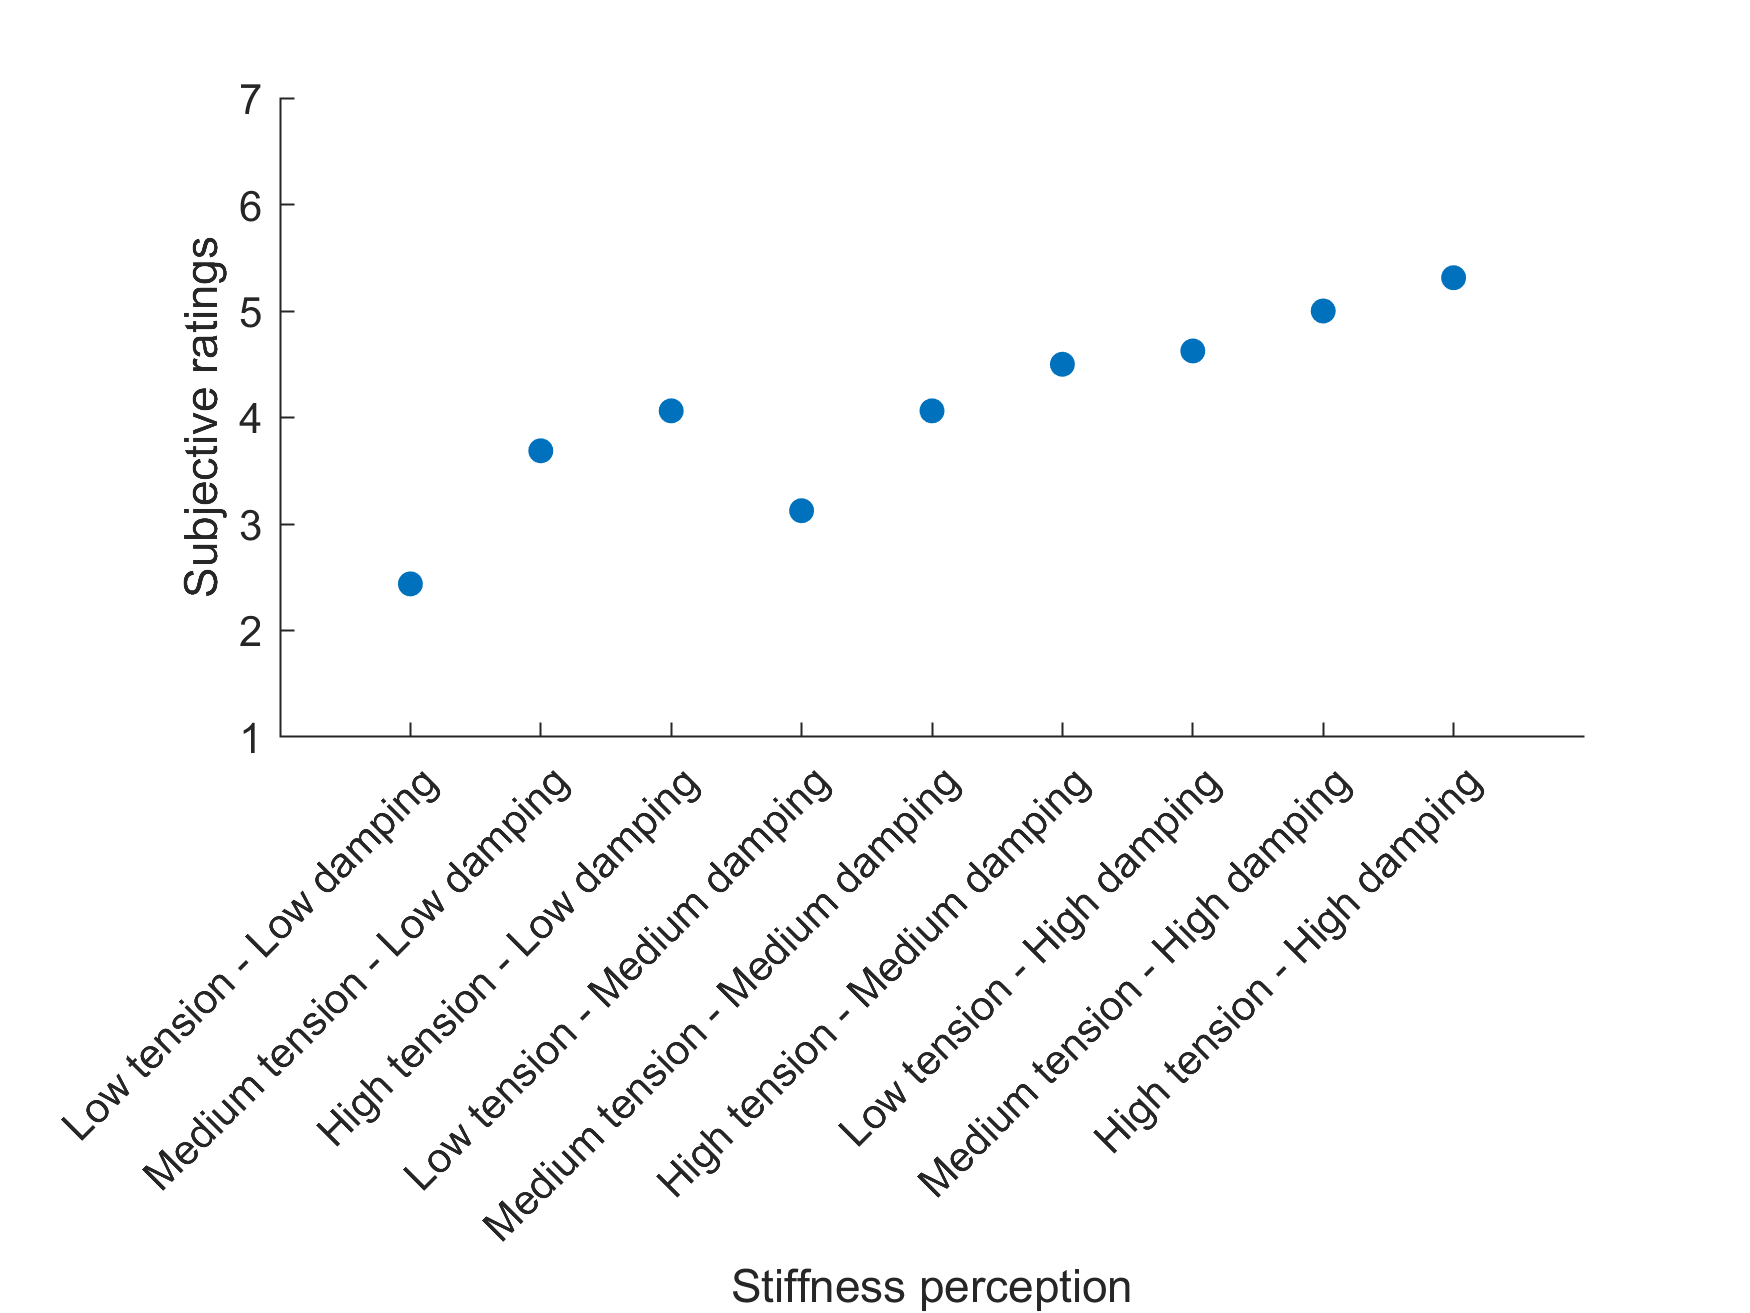
\includegraphics[width=0.5\textwidth]{Images/corr_anal}
\caption{Relation between stiffness perception and subjective ratings.}
\centering
\label{fig:results}
\end{figure} 
We can observe a quasi-linear relationship between subjective stiffness perception and the values for tension and damping used by the simulation. %It should be noted how lower values of stiffness (between 2 to 4) deviate from the linear trend: subjects had more uncertainty when they had to evaluate lower levels of membrane stiffness. \textbf{this was still assuming that the 9 cases were sorted by stiffness}

\autoref{fig:averagedResults} shows the average participant scores for each level of damping and tension. These two parameters were grouped in levels (low, medium and high) and subjective rankings are plotted as coloured bars. As previously hypothesised, the ratings of material stiffness increases with tension and damping.
\begin{figure}[t]
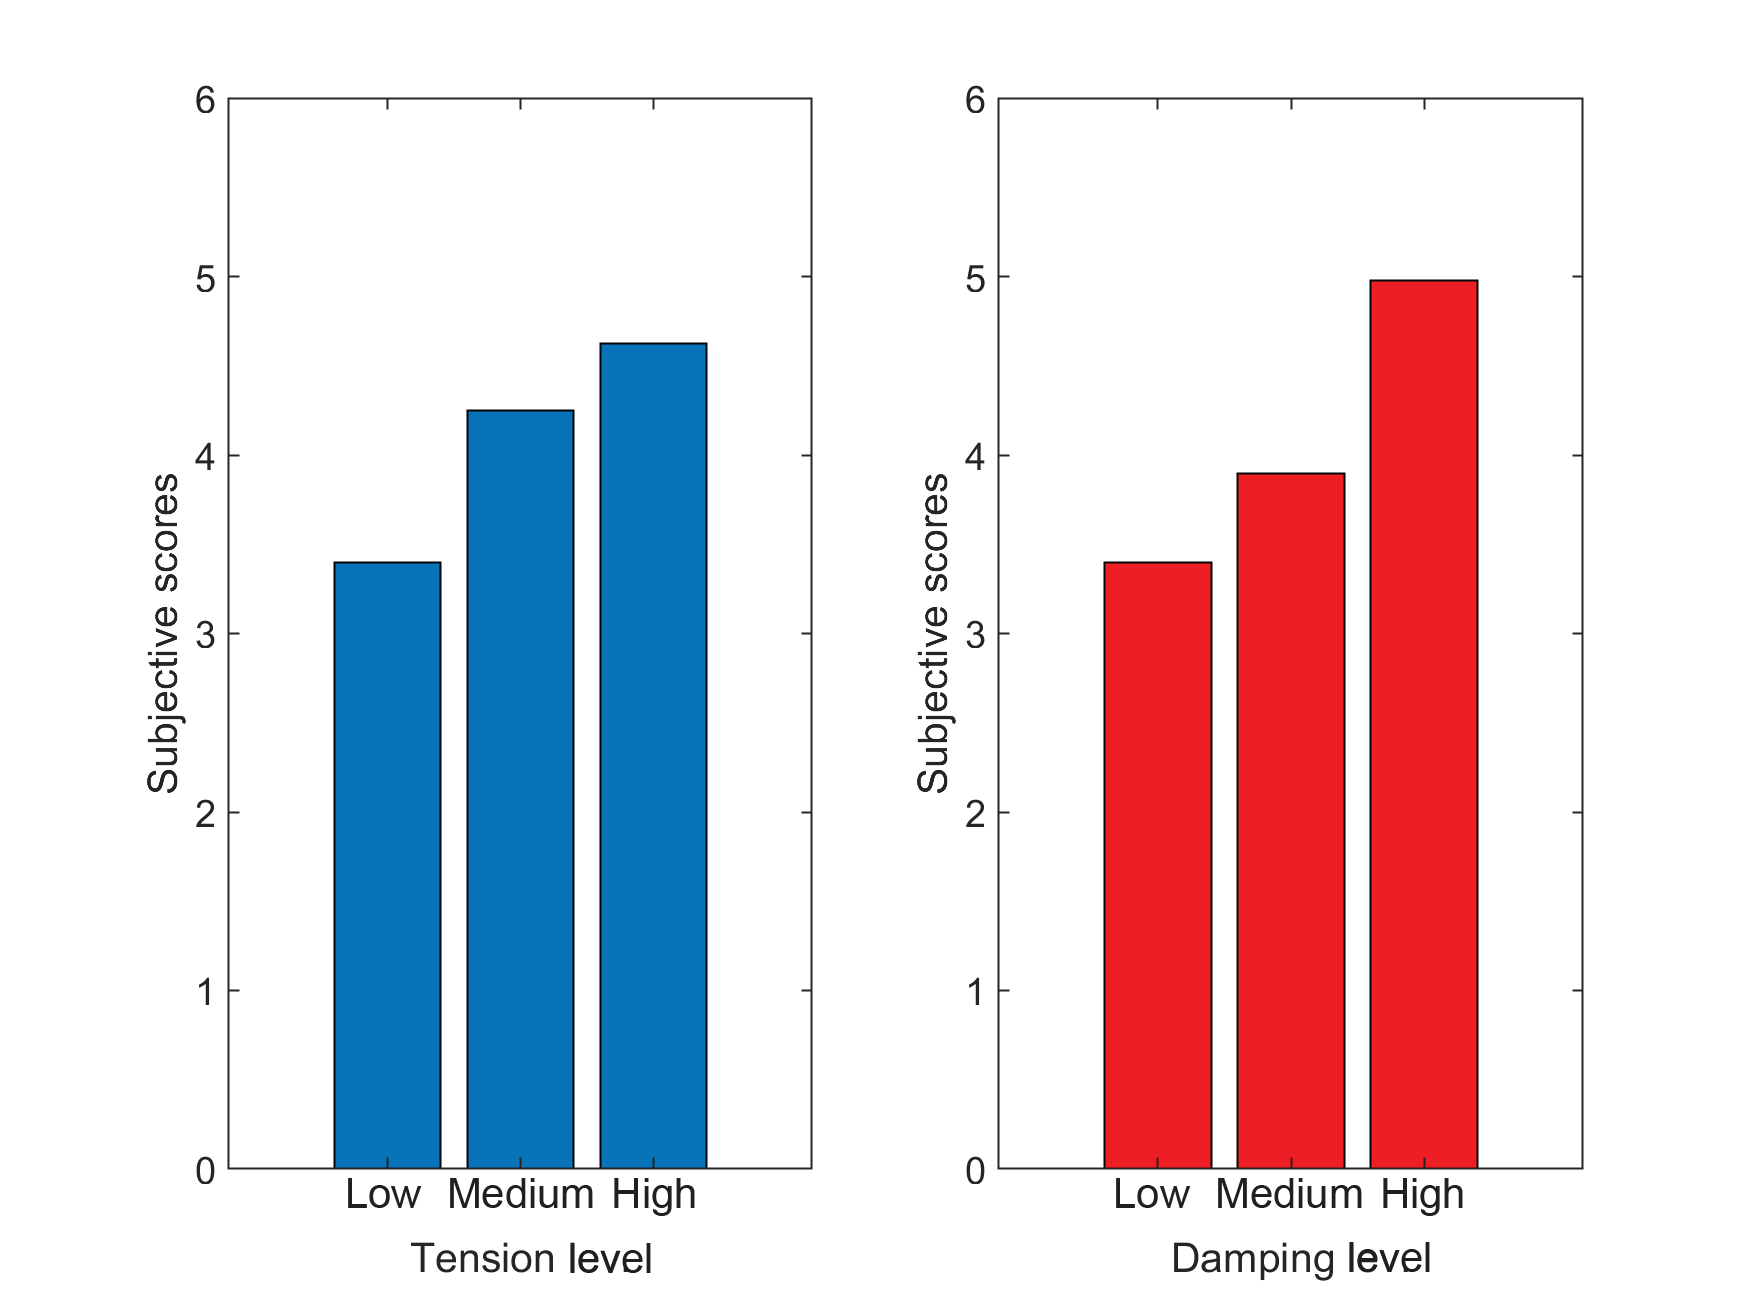
\includegraphics[width=0.5\textwidth]{Images/tens_dump}
\caption{Subjective ratings grouped by different tension and damping levels.}
\centering
\label{fig:averagedResults}
\end{figure} 
%\textbf{We also ran a group level statistical analysis using the Mann-Whitney U-test between tension and damping levels.} \textbf{\textleftarrow Something more about this?}

We also ran a statistical analysis on each single level based on non-parametric Mann-Whitney U-test and report the results in \autoref{tab:utest}. Abbreviations are T for ``tension" and D for ``damping" while letters L, M and H mean the levels ``low", ``medium" and ``high". It is important to take into account the multi-comparison problem and in this case the threshold level for significance should be equal to 0.0056 following the Bonferroni correction.

\def \columnW {0.33cm}
\begin{table}[h!]
\tiny
\caption{Mann-Whitney U-test (p-values).}
\begin{tabular}{ |p{0.7cm}||p{\columnW}|p{\columnW}|p{\columnW}|p{\columnW}|p{\columnW}|p{\columnW}|p{\columnW}|p{\columnW}|p{\columnW}|  }
 \hline
 \multicolumn{10}{|c|}{Mann-Whitney U-test [p values]} \\
 \hline
  & LT LD & MT LD & HT LD & LT MD & MT MD & HT MD & LT HD & MT HD & HT HD \\
 \hline
LT LD &	 &.0642 &.0163 &.1268 &.0049 &.0041 &.0034 &.0004 &.0002\\
\hline
MT LD &.0642 &	 &.6463 &.3465 &.6582 &.1802 &.1584 &.034 &.0091\\
\hline
HT LD &.0163 &.6463 &	 &.2123 &.8933 &.5413 &.4455 &.1737 &.0915\\
\hline
LT MD &.1268 &.3465 &.2123 &	 &.0791 &.0254 &.0283 &.0012 &.0009\\
\hline
MT MD &.0049 &.6582 &.8933 &.0791 &	 &.3191 &.3114 &.0449 &.0174\\
\hline
HT MD &.0041 &.1802 &.5413 &.0254 &.3191 &	 &.7732 &.5214 &.1383\\
\hline
LT HD &.0034 &.1584 &.4455 &.0283 &.3114 &.7732 &	 &.7725 &.3424\\
\hline
MT HD &.0004 &.034 &.1737 &.0012 &.0449 &.5214 &.7725 &	 &.2991\\
\hline
HT HD &.0002 &.0091 &.0915 &.0009 &.0174 &.1383 &.3424 &.2991 &	\\

 \hline
 \multicolumn{10}{|c|}{Note: Bonferroni adjusted significance threshold for multi-comparison p\textless0.0056} \\
 \hline
\end{tabular}
\label{tab:utest}
\end{table}

As we can observe from \autoref{tab:utest}, there isn't a significant difference between ``high tension -- low damping" and ``low tension -- medium damping" (p = 0.2123) suggesting that the linear relation of Figure 7 holds despite the discontinuity between points as seen on the scatterplot. However, we should consider it similar to a monotonically increasing function rather than a pure linear trend. 

Lastly, \autoref{tab:groupComp} shows group comparisons between the three different values of damping and tension. 
\begin{table}[t]
\centering
\caption{Comparison between different levels of tension and damping.}\label{tab:groupComp}
\begin{tabular}{ |c|c|c| } 
 \hline
 \multicolumn{2}{| c |}{Different levels of tension/damping} & p-values\\
 \hline
 Low Damping & Medium Damping & 0.2560 \\ 
 Medium Damping & High Damping & 0.0078 \\
 Low Damping & High Damping & 6.5071e-04 \\
 Low Tension & Medium Tension & 0.0950 \\
 Medium Tension & High Tension & 0.4268 \\
 Low Tension & High Tension & 0.0297 \\
 \hline
\end{tabular}
\end{table}
We notice a significant difference in participant's ratings between medium-high damping and low-high damping levels while tension shows significance only between low to high tension. We can deduct from the results that damping is a more important factor than tension in material stiffness perception. This result is slightly unexpected, as it was previously hypothesised that tension would be the most dominant factor in stiffness perception. Another observation is that it appears difficult for participants to evaluate low to medium levels of both damping and tension. In a future test, the values could be differently chosen, or more alternatives for the parameter values could be investigated to better see the perceptual differences between these values. 

\subsection{Statistical Analysis: Reliability}
Individual ratings were initially analysed with Cronbach's alpha \cite{Cronbach1951} to test the internal consistency of the responses. This measure is generally known as a metric to validate a questionnaire with higher values of alpha as those more desirable. The non-standardised Cronbach's alpha value was 0.6348 while the standardised value reached 0.6589. According to \cite{Kline2000}, a value between 0.6 to 0.7 is questionable (questionnaire scale is not fully reliable) with 0.7 as the threshold for an acceptable test. Despite the outcomes being slightly below threshold (probably caused by subjective difficulties in evaluating stiffness), it appears that in future we could easily reach a good reliability by increasing the sample size. Moreover, if we don't consider all factors loadings as evenly distributed, we could assume that the Cronbach's alpha underestimates the true reliability. 

\subsection{Questionnaire}
As can be seen from the questionnaire results in \autoref{tab:results} the participants generally found that the hands in the simulation were their own. This proves that the Leap Motion is a good way to track the hands and that it was well implemented. Moreover, it is clear that the visuals had no influence on participants' judgement, most probably because they were unchanged. The audio, however, seemed to be the most predominant feature that the users focused on when expressing their judgements (93.8\%). Haptics for expressing judgements was only chosen by 5 participants (31.3\%). In the future, removing the audio, only leaving the haptics might be a better way to force the user to use their sense of touch and test the influence of this modality on perception.

\begin{table}[t]
\small
\caption{Questionnaire results. The last two questions were taken from \cite{avanzini2006}.}\label{tab:results}
\centering
\begin{tabular}{|p{6cm}|p{1.5cm}|}
    \hline
    Question & Result \\
    \hline
    \vspace{0.05em}
    I felt like the hands in the simulation were my & \vspace{0.05em}$\mu = 5.44$,\\
    own. (1-7 rating) & $\sigma = 1.26$ \\
    & \\
    In order to express your judgements to the ques- & visuals: \, 0,\\
    tions during the simulation, you relied mainly & audio: \: 15, \\ on... (visuals\textbar audio\textbar haptics) & haptics: \: 5 \\
    &\\
    In your opinion what was varying between each & visuals: \, 0, \\
    condition? (visuals\textbar audio\textbar haptics) & audio: \: 14,\\
    & haptics: 10 \\
    \hline
\end{tabular}
\end{table}

\subsection{Other Observations}
From participant observation during the experiment, comments they gave during and after the test, and the two last (open) questions of the questionnaire (see Section \ref{sec:exp}) we obtained some extra findings. 

Due to the fact that the virtual drum was placed slightly higher than the physical drum (see Section \ref{sec:sys}), many participants interacted with the air above the drum rather than finishing their stroke to actually hit the drum. This was an issue, as the haptic sensation would not be felt in that case. This might also explain the result of the second question in \autoref{tab:results}. Either before or during the test, the participants were instructed to finish their stroke to actually physically interact with the drum. 

The interaction was programmed in such a way, that when a tracked hand collides with the virtual drum, this hand would not be able to trigger the physical model until it was completely out of the ``collision zone". Due to the misalignment mentioned above, many interactions were not captured. Again, either before or during the experiment, the participants were instructed to make longer movements to ensure that their hands were completely outside of this ``collision zone" before interacting with the drum again.

Another technical issue was that sometimes participants would look forward rather than down to the hands. This caused the hands not to be tracked anymore as the Leap Motion was mounted on the HMD. A solution for this would be to mount it at a lower angle rather than straight forward (as is the case now).

The experiment could be improved by addressing the above interaction issues to yield stronger data. The issues could potentially be solved by adding a more precise sensor to the setup, such as placing a contact microphone on the drum membrane. Even though a feedback loop could occur due to the haptuator being present on the same membrane, there is a potential to filter out and only use the transients (interaction with the membrane) for control.

Some participants commented that they would have liked to have reference points for ``the stiffest" and ``the softest" cases before testing as they said they would have judged the first few cases differently if they had known these references in advance. This could, however, bias the participants' answers.

The movements of participants were observed during the test and sporadically noted. There was a small tendency towards slower and longer movements in the case of lower tension and faster and shorter movements in the opposite case, but as these observations were not done systematically, to be able to say anything about this, this should be properly tested, possibly using raw data from the hand tracking.

%The physical model of the membrane allows for sound experimentation with sounds which 
%In this paper we presented a setup made of: a virtual reality drum which involves a physical prop providing haptic feedback. Considering that different physical drums would produce different acoustic results and a musician would have to spend hours practicing and improving their stroke techniques for a specific one - our virtual reality musical instrument is an implementation of 3 different drum types into a single setup. While getting the haptic feedback of a drumming experience, one can switch between different musical instruments, explore their potential and train their stroke. This takes advantage of the fact that VR allows for possibilities which could not happen in the real world.

\section{Conclusion}\label{sec:conc}

In this paper, we presented and evaluated a novel VRMI where a physical drum was enhanced by VR. The physical drum was augmented by a vibration motor and the sound was simulated using a physical model of a drum membrane. In an experiment run during the study, preliminary results show that higher values for both tension and damping increase the perception of material stiffness of the drum membrane, as hypothesised. However, the damping appeared to be a more important factor in this perception than the tension, which was contrary to our expectations. Improving the experiment by, for example, adding a contact microphone to the membrane for more accurate control and reconducting the experiment with a larger sample size will be necessary to validate or improve the results presented in this paper.

Other future work includes decoupling the audio and the haptics, to test the perceptual influence of each individual modality separately. Also, more alternatives of the parameter values could be presented in a future test to more deeply investigate the connection between parameter values and stiffness perception.

Additionally, the tracking of the user's hands should be improved by mounting the Leap Motion more downwards on the HMD. Furthermore, the virtual and physical drum should be better aligned in space as to make the interaction less confusing and more intuitive.
Lastly, in order to test whether the interaction patterns change depending on the changes in parameters, the raw data from the hand tracking should be analysed. As an addition to this, the Myo armband could be used to get more complex interaction data.

%% if specified like this the section will be committed in review mode
\acknowledgments{
The authors wish to thank Stefania Serafin, Cumhur Erkut, Niels Nilsson, Rolf Nordahl, and Michele Geronazzo -- our teachers of the ``Virtual, Augmented, Mixed realities" PhD course at Aalborg University Copenhagen for their help during the process of this project.}
%%%%%%%%%%%%%%%%%%%%%%%%%%%%%%%%%%%%%%%%%%%%%%%%%%%%%%%%%%%%%%%%%%%%%%%%%%%%%
%bibliography here
\bibliography{smc2020bib}

\end{document}
